%\documentclass[conference]{IEEEtran}
\documentclass[12pt]{article}
\usepackage{graphicx,cite,bm,psfrag,amsmath}
\def\mmax{\mathop{\mbox{\scriptsize max}}}
\def\argmin{\mathop{\mbox{arg\,min}}}
\def\argmax{\mathop{\mbox{arg\,max}}}
\newcommand{\defequal}{\stackrel{\mathrm{def}}{=}}
\renewcommand{\vec}[1]{{\ensuremath{\boldsymbol{#1}}}}
\newcommand{\popt}{\ensuremath{P^{(K)}_{opt}}}

%\pagestyle{plain}
\usepackage{amsfonts}
\usepackage{algorithm, algorithmic}
\renewcommand{\algorithmicrequire}{ \textbf{Input:}} %Use Input in the format of Algorithm
\renewcommand{\algorithmicensure}{ \textbf{Procedures:}} %UseOutput in the format of Algorithm
% correct bad hyphenation here
%\hyphenation{op-tical net-works semi-conduc-tor}
\usepackage{CJK}
\usepackage{color}
\usepackage{url}
\usepackage{geometry}
\geometry{left=0.55in, right=0.7in, top=0.75in, bottom=0.75in}

\begin{document}

%\begin{document}
%	\title{SIR-Based Power Control Used in CDMA Systems}
%	\author{
%	
%	\maketitle \thispagestyle{plain}
%	\pagenumbering{gobble}
 

\title{ Proof for The Matrix of Uplink Is The Transpose of Downlink} 
\date{}
\maketitle	
%\begin{abstract}
%	
%\end{abstract}

\section{In BS-to-BS Matrix}
We assume N base stations, and a common channel. Let $L_i$ denote the user number of cell i. We define a geometry as show in Fig. \ref{fig:t }, where $g_{ikj}$ denotes the gain for user k in cell i to base station in cell j.% Let $p_i^U$ denote the received power by the BS of the i-th cell from any one users in this cell, so that the power vector is \begin{equation*}
%\bm P^U = \left[ \begin{matrix}
%p_1^U,p_2^U,\cdots,p_N^U
%\end{matrix}\right]^T 
%\end{equation*}
% The signal to interference ration can be expressed as:
%
%\begin{equation}
%\gamma_i^U = \frac{p_i^U}{\sum_{j=1}^N p_j^U \sum_{k=1}^{L_j} \frac{ g_{jki} }{g__{jkj}}}-p_i^u}
%\end{equation}


\begin{figure*}[th]
	\centering
	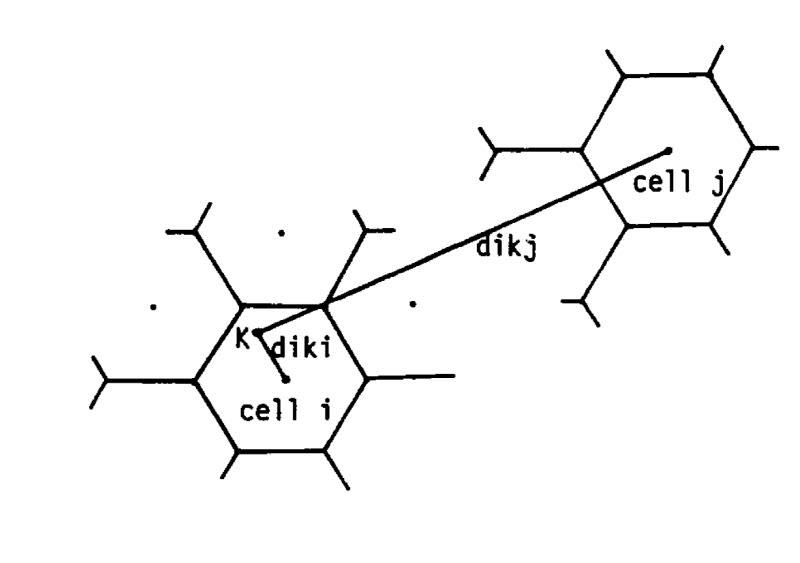
\includegraphics[width=0.7\linewidth]{t}
	\caption{Interference Geometry}
	\label{fig:t }
\end{figure*}

\subsection{SIR in Uplink}

Let $p_i^U$ denote the received power by the BS of the i-th cell from any one users in this cell, so that the power vector is \begin{equation*}
\bm P^U = \left[ \begin{matrix}
p_1^U,p_2^U,\cdots,p_N^U
\end{matrix}\right]^T. 
\end{equation*}
The signal to interference ration can be expressed as:

\begin{equation}
\gamma_i^U = \frac{p_i^U}{\sum\limits_{j=1}^N p_j^U \sum\limits_{k=1}^{L_j} \frac{ g_{jki} }{g__{jkj}}}-p_i^u}.
\end{equation}

Thus, \begin{equation*}
G^U=[G_{ij}^U];
\end{equation*}
where \begin{equation}
G_{ij}^U = \sum^{L_j}_{k=1} \frac{g_{jki}}{g_{jkj}}.
\end{equation}

\subsection{SIR in Downlink}

Then we assumed $p_{ik}^D$ as the transmit power at BS of cell i to the k-th user in the same cell. So that the desired signal of which user received is \begin{equation*}
p_{desired}= p_{ik}^D \times g_{iki}.
\end{equation*}

And $Q_i$ represents the total transmit power for the i-th BS. Thus, we can get that
\begin{equation}
Q_i= \sum_{k=1}^{L_i} p_{ik}^D.
\end{equation}
so that the power vector in the downlink is \begin{equation*}
\bm Q = \left[ \begin{matrix}
Q_1,Q_2,\cdots,Q_N
\end{matrix}\right]^T. 
\end{equation*}

The SIR at the user k in cell i can be expressed as:
\begin{equation}
\gamma_{ik}^D= \frac{p_{desired} }{\sum\limits_{j=1}^N Q_jg_{ikj}-p_{desired}} = \frac{p_{ik}^D g_{iki}}{\sum\limits_{j=1}^N Q_jg_{ikj}-p_{ik}^D g_{iki}}
\end{equation}
By the global power control algorithm, we should set  $\gamma_i^D$ = $\gamma_{ik}^D$ (i=1,2,\dots,N). Generally, the SIR values are different form cell to cell, and within a given cell, the SIR will be different between uplink and downlink. Also by the global PCA, we need to balance the values of SIR in the downlink for each cell. Setting all $\gamma_i^D$to be equal leads to an eigenvalue equation problems, which is same like uplink. Hence,



\begin{align*}
\gamma_i^D&=\frac{\sum p_{desired} }{\sum\limits_{j=1}^N Q_j \sum\limits_{k=1}^{L_i} g_{ikj}-\sum p_{desired}}\\   
&=\frac{\sum p_{ik}^D g_{iki} } {\sum\limits_{j=1}^N Q_j \sum\limits_{k=1}^{L_i} g_{ikj}-\sum p_{ik}^D g_{iki}}\\
&=\frac{\sum p_{ik}^D  } {\sum\limits_{j=1}^N Q_j \sum\limits_{k=1}^{L_i} \frac{g_{ikj}}{g_{iki}}-\sum p_{ik}^D}
\end{align*}
By (3) we can get the SIR values of downlink is \begin{equation}
\gamma_i^D=\frac{Q_i  } {\sum\limits_{j=1}^N Q_j \sum\limits_{k=1}^{L_i} \frac{g_{ikj}}{g_{iki}}-Q_i}
\end{equation}

Thus,  \begin{equation*}
G^D=[G_{ij}^D];
\end{equation*}
where \begin{equation}
G_{ij}^D = \sum^{L_i}_{k=1} \frac{g_{ikj}}{g_{iki}}.
\end{equation}

\subsection{result}

Now, we list the matrix of uplink and downlink,
\begin{equation}
\bm G^U = \left[ \begin{matrix}
\sum\limits_{k=1}^{L_1}\frac{g_{1k1}}{g_{1k1}}&\sum\limits_{k=1}^{L_2}\frac{g_{2k1}}{g_{2k2}}&\cdots&\sum\limits_{k=1}^{L_N}\frac{g_{Nk1}}{g_{NkN}}\\
\sum\limits_{k=1}^{L_1}\frac{g_{1k2}}{g_{1k1}}&\sum\limits_{k=1}^{L_2}\frac{g_{2k2}}{g_{2k2}}&\cdots&\sum\limits_{k=1}^{L_N}\frac{g_{Nk2}}{g_{NkN}}\\
\vdots&\vdots&\ddots&\vdots\\
\sum\limits_{k=1}^{L_1}\frac{g_{1kN}}{g_{1k1}}&\sum\limits_{k=1}^{L_2}\frac{g_{2kN}}{g_{2k2}}&\cdots&\sum\limits_{k=1}^{L_N}\frac{g_{NkN}}{g_{NkN}}
\end{matrix}\right]. 
\end{equation}
\begin{equation}
\bm G^D = \left[ \begin{matrix}
\sum\limits_{k=1}^{L_1}\frac{g_{1k1}}{g_{1k1}}&\sum\limits_{k=1}^{L_1}\frac{g_{1k2}}{g_{1k1}}&\cdots&\sum\limits_{k=1}^{L_1}\frac{g_{1kN}}{g_{1k1}}\\
\sum\limits_{k=1}^{L_2}\frac{g_{2k1}}{g_{2k2}}&\sum\limits_{k=1}^{L_2}\frac{g_{2k2}}{g_{2k2}}&\cdots&\sum\limits_{k=1}^{L_2}\frac{g_{2kN}}{g_{2k2}}\\
\vdots&\vdots&\ddots&\vdots\\
\sum\limits_{k=1}^{L_N}\frac{g_{Nk1}}{g_{NkN}}&\sum\limits_{k=1}^{L_N}\frac{g_{Nk2}}{g_{Nk2}}&\cdots&\sum\limits_{k=1}^{L_N}\frac{g_{NkN}}{g_{NkN}}
\end{matrix}\right]. 
\end{equation}
The equations (7) and equation (8) reveals that 
\begin{equation*}
G^U\quad=\quad\left[G^D\right]^T.
\end{equation*}


\end{document}